\documentclass[a4paper,10pt]{article}
\usepackage{fontspec}
\setmainfont[Path=fonts/,BoldFont=FandolSong-Bold.otf,ItalicFont=FandolSong-Regular.otf]{FandolSong-Regular.otf}
\XeTeXlinebreaklocale "zh"
\XeTeXlinebreakskip=0pt plus 1pt
\usepackage[left=24mm,right=24mm,top=22mm,bottom=22mm]{geometry}
\usepackage{graphicx,float,booktabs,array,caption,titlesec,fancyhdr,indentfirst}
\usepackage[hidelinks,unicode]{hyperref}
\hypersetup{pdfauthor={},pdftitle={订单流水与公开评价融合的小微商户经营收缩识别},pdfsubject={赛题三数据分析报告}}
\renewcommand{\normalsize}{\fontsize{10.5bp}{15.75bp}\selectfont}
\normalsize
\setlength{\parindent}{21bp}
\setlength{\parskip}{0pt}
\setlength{\tabcolsep}{4pt}
\newlength{\tablewidth}
\renewcommand{\arraystretch}{1.05}
\setlength{\textfloatsep}{6pt}
\setlength{\intextsep}{6pt}
\captionsetup{labelformat=empty,font=normalsize,skip=3pt}
\titleformat{\section}{\normalfont\fontsize{12pt}{18pt}\selectfont\bfseries}{}{0pt}{}
\titlespacing*{\section}{0pt}{6pt}{4pt}
\pagestyle{fancy}
\fancyhf{}
\fancyfoot[C]{\fontsize{9pt}{12pt}\selectfont\thepage}
\renewcommand{\headrulewidth}{0pt}
\setlength{\headheight}{0pt}
\setlength{\footskip}{12mm}
\emergencystretch=1em
\begin{document}
\begin{titlepage}
\centering
\vspace*{30mm}
{\fontsize{15pt}{23pt}\selectfont 2026 FinTechathon 深圳国际金融科技大赛\par}
\vspace{5mm}
{\fontsize{12pt}{18pt}\selectfont 数据分析赛道 · 赛题三\par}
\vspace{26mm}
{\fontsize{20pt}{30pt}\selectfont\bfseries 订单流水与公开评价融合的小微商户经营收缩识别\par}
\vspace{5mm}
{\fontsize{13pt}{21pt}\selectfont ——基于真实交易的时间外验证与复核决策\par}
\vspace{30mm}
{\fontsize{14pt}{21pt}\selectfont 小组名称：285小组\par}
\end{titlepage}
\setcounter{page}{1}
\normalsize
\section*{摘要}
针对小微主体经营数据稀疏的问题，本文采用数据提供方公开的真实电商交易样本，以订单流水构建基线，加入评价及履约信息，检验增量和有限预算复核价值。原始数据含99,441笔订单、112,650条商品明细及99,224条评价；构建17项指标，按季度观察点训练、验证并留出未来90天标签。主测试包含581家商户，229家未来平台订单销售额下降至少50\%。增强组合AP为0.558，较交易基线增加0.0103，95\%配对区间为[-0.007，0.027]，尚未证明稳定增益。复核59家时交易基线和增强组合均命中42家，低评分策略命中27家；更晚观察点也未确认增强优势。结果支持交易信息用于经营收缩调查排序，公开评价先用于核查解释，不宜强行加分。订单金额不等于银行净现金流，未来平台收缩不是停业或信用违约；本研究属于历史时间外回测。

关键词：公开数据；订单流水；未来经营收缩；时间外验证；复核决策

\section*{一、业务背景与研究问题}
小微主体通常缺少标准化报表，交易记录能反映经营规模和波动，公开口碑则可能补充消费体验与履约线索。但评价是否有价值，应在已有交易基线上检验，而不是把差评直接等同风险。本文研究：交易指标能否识别未来平台经营收缩？评价与履约是否增加识别价值？固定核查预算下是否值得增加数据成本？

本研究将电商商户作为信息稀疏经营主体的代理，不声称已确认其小微规模。以未来90天订单销售额收缩作为可验证的经营风险线索，使用真实交易而非模拟流水。公开信息与交易来自同一数据提供方，是模块增量检验，尚非独立外部平台与银行流水的融合验证。


\newpage
\section*{二、公开数据、清洗与样本}
数据来自提供方官方公开仓库[1]，固定提交及文件SHA256见复现清单。README说明这些关系表直接抽样自交易系统；仓库附MIT许可证[2]，报告保留来源，原始消费者记录和逐商户数据不公开。商户、订单、商品明细和评价通过ID关联，不做跨来源猜测匹配。

\begin{table}[H]
\centering
\caption{表1 数据字段、规模与处理规则}
\setlength{\tablewidth}{\linewidth}
\addtolength{\tablewidth}{-6\tabcolsep}
\begin{tabular}{>{\raggedright\arraybackslash}p{0.180\tablewidth}>{\raggedright\arraybackslash}p{0.180\tablewidth}>{\raggedright\arraybackslash}p{0.640\tablewidth}}
\toprule
\textbf{数据表} & \textbf{原始记录数} & \textbf{字段与处理} \\
\midrule
订单 & 99,441 & 批准、配送和预计送达时间；不输入当前最终状态 \\
商品明细 & 112,650 & 商户ID、订单ID、价格；按商户—订单汇总价格 \\
评价 & 99,224 & 评分、回答时间；只用观察日前已回答评价 \\
商户 & 3,095 & 匿名商户ID、地区；地区仅作敏感性核对 \\
\bottomrule
\end{tabular}
\end{table}
订单缺失批准时间160笔，无法定位交易时点，排除其关联交易；商品明细均匹配订单。复核发现61笔配送早于批准，将配送时间记为未知；20条评价早于批准，剔除。1,278笔多商户订单的评价不能可靠归因，评价特征只用单商户订单，交易仍按实际商户明细分配。批准交易时间覆盖2016年9月至2018年9月。

\begin{figure}[H]
\centering
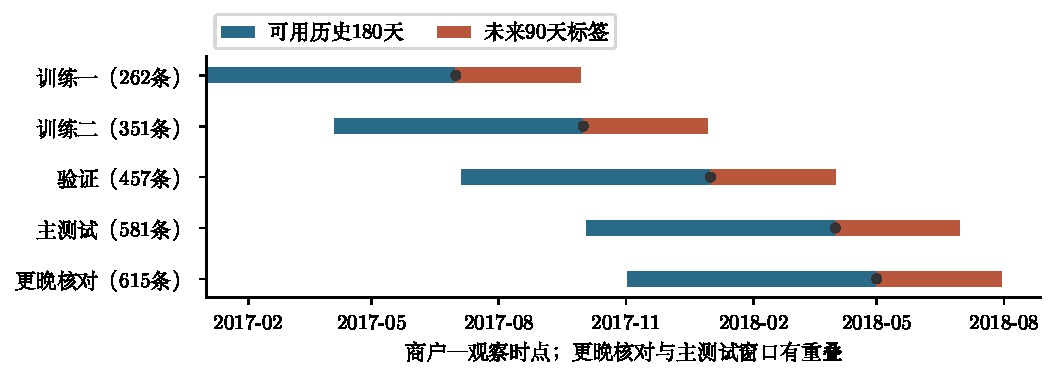
\includegraphics[width=1\linewidth]{figures/figure01_timeline.pdf}
\caption{图1 历史可用窗口与未来标签窗口；更晚核对并非独立复验}
\end{figure}
仅按观察日前条件纳入：过去180天订单≥10笔、近90天≥3笔、首笔交易至少早于观察日90天。主测试期近180天有交易商户1,686家，纳入581家，覆盖34.46\%；低频、新进入或信息不足商户另行补资料，不能默认为低风险。


\newpage
\section*{三、指标机制与描述性分析}
交易指标T衡量经营规模、变化和稳定性；评价Q反映消费者体验；履约L提供交付质量和积压线索。机制假设是体验与交付问题可能影响复购和经营，但这种关系受规模、季节性和平台结构影响，必须验证而不硬编码风险方向。

\begin{table}[H]
\centering
\caption{表2 交易、评价与履约指标体系（17项）}
\setlength{\tablewidth}{\linewidth}
\addtolength{\tablewidth}{-6\tabcolsep}
\begin{tabular}{>{\raggedright\arraybackslash}p{0.170\tablewidth}>{\raggedright\arraybackslash}p{0.430\tablewidth}>{\raggedright\arraybackslash}p{0.400\tablewidth}}
\toprule
\textbf{模块} & \textbf{指标} & \textbf{口径与机制} \\
\midrule
T：交易9项 & 180/90天金额与订单数；金额/订单变化；月度金额变异系数；客单价；距最后订单天数 & 批准订单商品价之和；变化用log(1+近期)-log(1+前期)，衡量经营动态 \\
Q：评价5项 & 均分、低分占比、评分标准差、近期均分变化、评价覆盖率 & 仅观察日前已回答的单商户订单评价；低分≤2分，反映体验线索 \\
L：履约3项 & 已知延期占比、已知配送天数、未确认完成占比 & 只按当时已发生的配送时间判断；后来配送不提前视为已完成 \\
\bottomrule
\end{tabular}
\end{table}
金额不含运费，不等于客户总支付、商户结算收入或净现金流，退款和取消历史不可得。评价使用回答时间而非问卷创建时间；同订单多次评价只取当时最新回答。评分变化按订单所属近期/前期窗口计算；无评价或配送记录时保留缺失，仅在拟合数据中估计中位数并增加缺失指示。

\begin{figure}[H]
\centering
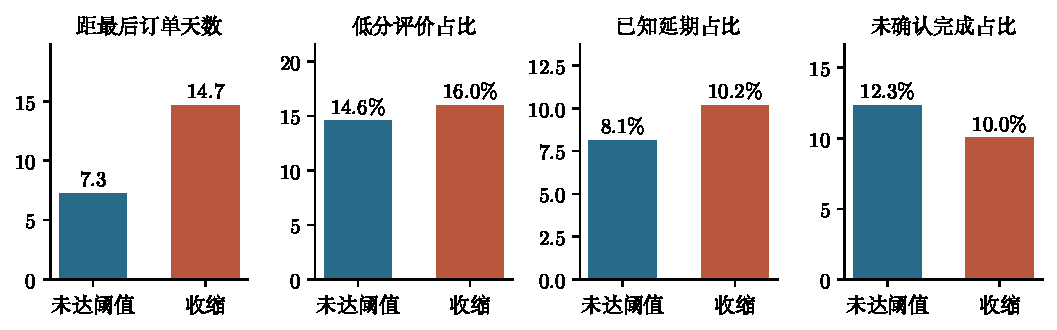
\includegraphics[width=1\linewidth]{figures/figure02_profiles.pdf}
\caption{图2 主测试期商户的历史指标均值（按未来收缩标签分组）}
\end{figure}
未来收缩组距最后订单均值为14.67天，未达阈值组7.25天；低分占比分别为16.00\%和14.59\%。未确认完成比例的方向并不符合简单“越高越危险”的假设。以上仅作描述，不证明因果或独立增量。


\newpage
\section*{四、未来标签与时间外验证}
统一月末观察，特征只用观察日及之前180天可获得事件。未来90天商品销售额记为G未来，过去90天记为G历史，主标签为G未来≤0.5×G历史。标签代表平台内显著经营收缩，包含可能的平台迁移或正常波动；不称为真实财务困境、停业或违约。门槛在建模前固定，并用下降≥70\%与≥30\%定义作敏感性分析。

\begin{table}[H]
\centering
\caption{表3 时间划分、样本与标签成熟}
\setlength{\tablewidth}{\linewidth}
\addtolength{\tablewidth}{-8\tabcolsep}
\begin{tabular}{>{\raggedright\arraybackslash}p{0.310\tablewidth}>{\raggedright\arraybackslash}p{0.180\tablewidth}>{\raggedright\arraybackslash}p{0.120\tablewidth}>{\raggedright\arraybackslash}p{0.390\tablewidth}}
\toprule
\textbf{阶段／观察日} & \textbf{商户—时点数} & \textbf{收缩数} & \textbf{标签区间} \\
\midrule
训练：2017-06-30 & 262 & 75 & 2017-07-01至09-28 \\
训练：2017-09-30 & 351 & 86 & 2017-10-01至12-29 \\
验证：2017-12-31 & 457 & 135 & 2018-01-01至03-31 \\
主测试：2018-03-31 & 581 & 229 & 2018-04-01至06-29 \\
更晚核对：2018-04-30 & 615 & 263 & 2018-05-01至07-29 \\
\bottomrule
\end{tabular}
\end{table}
训练613条商户—时点记录来自389家商户；验证457家。主测试一商户一条记录，训练标签在验证前成熟，验证标签在主测试观察日结束时成熟。相同商户可出现在不同阶段，检验的是以后时点而非随机商户划分；更晚核对与主测试商户及未来窗口重叠，不冒充独立复验。

比较LR逻辑回归与HGB梯度提升树，各含T、TQ、TQL三种输入。LR调C=0.1、1、10；HGB调叶节点7、15和L2=1、5，固定150次迭代、学习率0.05、每叶至少20条，不早停。只按验证AP调参，并按T基线验证AP选算法家族，再固定该家族比较公开信息增量。本次选择LR，TQL是主增量检验组合，并非验证最优部署方案。

最终模型用训练＋验证重拟合，预处理只在拟合数据学习；不用主测试标签调参。报告ROC-AUC、非插值AP、Brier及约10\%预算指标；2,000次配对商户Bootstrap覆盖固定模型的本次测试抽样不确定性，不涵盖训练重拟合和选择过程。更晚核对沿用同一固定模型，未加入主测试标签重训。


\newpage
\section*{五、交易基线与公开信息的增量}
\begin{figure}[H]
\centering
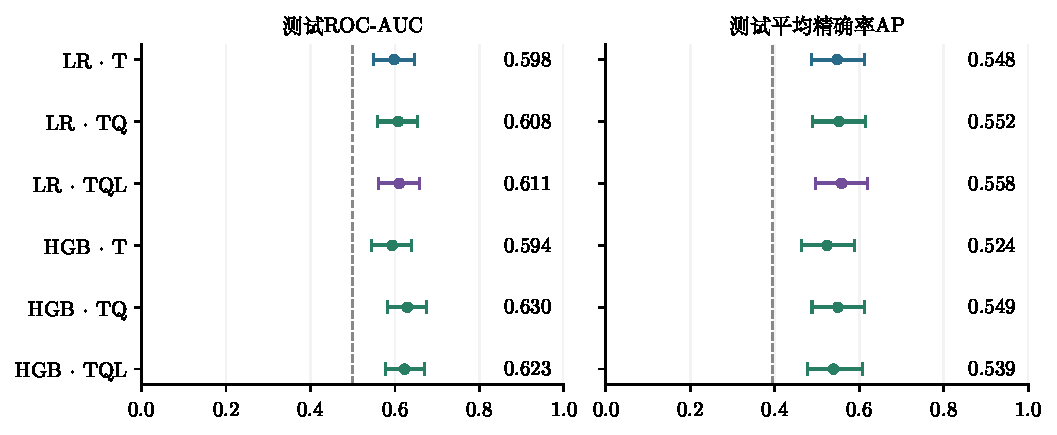
\includegraphics[width=1\linewidth]{figures/figure03_models.pdf}
\caption{图3 六个预设模型的测试表现及95\%配对Bootstrap区间}
\end{figure}
\begin{table}[H]
\centering
\caption{表4 验证及主测试结果（Brier越低越好）}
\setlength{\tablewidth}{\linewidth}
\addtolength{\tablewidth}{-10\tabcolsep}
\begin{tabular}{>{\raggedright\arraybackslash}p{0.260\tablewidth}>{\raggedright\arraybackslash}p{0.170\tablewidth}>{\raggedright\arraybackslash}p{0.190\tablewidth}>{\raggedright\arraybackslash}p{0.180\tablewidth}>{\raggedright\arraybackslash}p{0.200\tablewidth}}
\toprule
\textbf{模型} & \textbf{验证AP} & \textbf{测试AUC} & \textbf{测试AP} & \textbf{Brier} \\
\midrule
LR·T & 0.429 & 0.598 & 0.548 & 0.2406 \\
LR·TQ & 0.423 & 0.608 & 0.552 & 0.2399 \\
LR·TQL & 0.413 & 0.611 & 0.558 & 0.2390 \\
HGB·T & 0.399 & 0.594 & 0.524 & 0.2500 \\
HGB·TQ & 0.406 & 0.630 & 0.549 & 0.2431 \\
HGB·TQL & 0.387 & 0.623 & 0.539 & 0.2497 \\
\bottomrule
\end{tabular}
\end{table}
交易基线LR·T的测试AP为0.548，增强组合LR·TQL为0.558；AP增量0.0103，95\%区间[-0.007，0.027]包含0。AUC从0.598到0.611，差的区间也包含0。评价Q和履约L的点估计改善不能证明已提供稳定增益，未据测试最高分回头改选模型。

验证期T基线AP高于TQL增强，部署选择不能忽略这一结果。拟合期正例比例27.66\%，主测试39.41\%，存在分布变化。用拟合期比例作常数预测的测试Brier为0.2526，增强组合为0.2390；这属于概率评分比较，不证明概率已校准，更不能转称信用违约概率。


\newpage
\section*{六、应用验证：有限预算复核}
预先设定每期约10\%核查预算，581家向上取整复核59家（10.15\%）。名单按固定分数排序，不用未来标签选名单；低评分策略使用同一历史评价口径，并按预设匿名ID顺序处理并列。未来标签只用于事后核对调查优先级。

\begin{figure}[H]
\centering
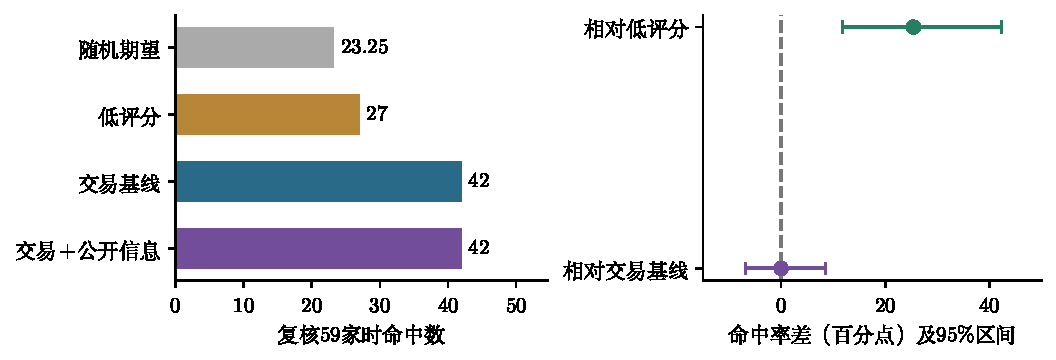
\includegraphics[width=1\linewidth]{figures/figure04_budget.pdf}
\caption{图4 固定预算命中数及增强组合相对两类基线的命中率差}
\end{figure}
\begin{table}[H]
\centering
\caption{表5 主测试复核预算效果}
\setlength{\tablewidth}{\linewidth}
\addtolength{\tablewidth}{-10\tabcolsep}
\begin{tabular}{>{\raggedright\arraybackslash}p{0.300\tablewidth}>{\raggedright\arraybackslash}p{0.160\tablewidth}>{\raggedright\arraybackslash}p{0.190\tablewidth}>{\raggedright\arraybackslash}p{0.190\tablewidth}>{\raggedright\arraybackslash}p{0.160\tablewidth}}
\toprule
\textbf{策略} & \textbf{命中数} & \textbf{命中率} & \textbf{捕获率} & \textbf{随机提升} \\
\midrule
随机期望 & 23.25 & 39.41\% & 10.15\% & 1.00 \\
低评分 & 27 & 45.76\% & 11.79\% & 1.16 \\
交易基线 & 42 & 71.19\% & 18.34\% & 1.81 \\
交易＋公开信息 & 42 & 71.19\% & 18.34\% & 1.81 \\
\bottomrule
\end{tabular}
\end{table}
增强组合相对低评分多命中15家，命中率差25.42个百分点，配对区间为[11.86，42.37]个百分点。但交易基线同样命中42家，增加公开信息的复核命中数增量为0，不能把交易优势归给评价模块。随机23.25家为理论期望。

增强名单仍漏掉81.66\%的未来收缩商户，因此不能用于排除未上榜主体的风险。这里只验证未来平台收缩线索的排序，不测真实违约、财务损失或处置收益；复核命中不能直接换算为节省金额。


\newpage
\section*{七、稳定性复核与适用边界}
\begin{figure}[H]
\centering
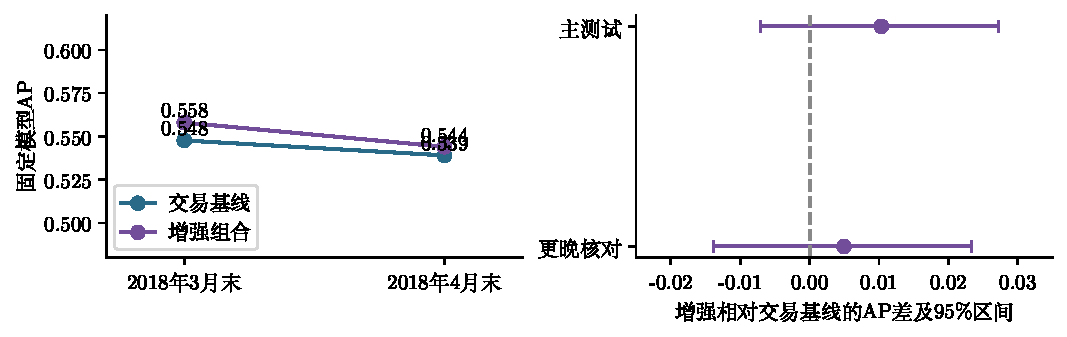
\includegraphics[width=1\linewidth]{figures/figure05_stability.pdf}
\caption{图5 固定模型跨观察点表现；两个窗口重叠，不能视为独立复验}
\end{figure}
更晚核对含615家商户，交易基线AP为0.539，增强组合0.544，增量区间[-0.014，0.023]仍包含0。两期增强增量均小，尚未证明稳定改善；更晚期AUC增强未优于交易基线。反复选择最有利月份或标签门槛会产生选择偏差，本研究保留所有核对结果。

按订单≥20、评价覆盖≥50\%、主要地区/其他地区及训练未出现商户进行固定预测核对；标签改为下降≥70\%时，增强AP没有优于基线，改为下降≥30\%时点估计增加。子组没有重新调参，也没有据此改主结论；阈值敏感性与地区核对不等于独立外推验证。

数据边界：数据提供方只发布平台抽样，不是全部经营额；未来无订单可能表示平台迁移、样本缺失或主动退出。价格及订单明细缺少事件版本，退款、取消历史不可得，无法完全还原历史结算状态。按时间戳重建可用信息比静态营业标签更严格，但仍是历史回测。

外推边界：商户规模未确认，海外2016—2018年电商数据不能证明2026年深圳线下小微主体适用。评价和履约同源，不能据此证明跨独立平台公开数据的增益。低频商户和新商户被门槛排除，应单独核查；全量漏报须有独立标签或带已知抽样概率的随机核查，不能只核查模型名单后声称召回率提高。


\newpage
\section*{八、产品思路与商业闭环}
建议产品定位为“商户经营线索助手”：用交易变化形成待调查名单，用公开评价及履约线索提示核查方向。当前证据优先支持交易基线排序，公开模块先作解释展示；不把未确认增量的模块强行叠加评分，不输出贷款违约概率。

\begin{table}[H]
\centering
\caption{表6 证据对应产品动作与验收}
\setlength{\tablewidth}{\linewidth}
\addtolength{\tablewidth}{-6\tabcolsep}
\begin{tabular}{>{\raggedright\arraybackslash}p{0.230\tablewidth}>{\raggedright\arraybackslash}p{0.340\tablewidth}>{\raggedright\arraybackslash}p{0.430\tablewidth}}
\toprule
\textbf{模块} & \textbf{已有证据} & \textbf{业务动作} \\
\midrule
可用性分流 & 主测试覆盖34.46\%活跃商户 & 未覆盖者补资料并保留随机核查 \\
交易调查排序 & 59家命中42家未来收缩 & 核实收入、退款及平台迁移，独立记录结果 \\
评价／履约画像 & 增量区间包含0；同预算未增加命中 & 展示真实历史指标及来源，不作为拒贷依据 \\
反馈与回退 & 尚无真实信用表现或处置成本 & 记录误报、失访、耗时及干预；效果不足暂停排序 \\
\bottomrule
\end{tabular}
\end{table}
商业验收设每期复核k家，p为经未来核实的可行动风险命中率，v为每次有效发现的处置净价值，c为单家核查成本，F为固定成本，则净价值=k×(p×v-c)-F。同预算增加公开模块的增量价值=(新增有效命中)×v-新增固定成本。本次增量命中为0，不能证明值得增加评分成本；画像是否节省核查时间需另行试点测量。

\section*{九、结论与下一步验证}
第一，真实订单基线与未来90天标签补强了研究契合度与时间方向，交易排序优于单纯低评分筛选。第二，公开评价及履约的增量仍未得到稳定证明；合理决策是将其作为核查线索，保留交易基线。第三，未来平台收缩不等于财务困境或违约，应在取得授权的真实结算流水和未来信用标签上复验。

后续在统一月末锁定真实流水基线、流水＋独立公开信息、10\%预算及成本口径，训练标签须在测试日前成熟；留出后续月份和新地区，保留随机核查对照。未知/失访不标为正常，干预效果单独评价，每月监测覆盖、命中和成本；仅在预设增量区间下界>0且净价值>0时扩大，否则回退人工核实。该闭环是待执行试点，不是已完成业务成果。


\newpage
\fancyfoot[C]{\fontsize{9pt}{12pt}\selectfont 参考文献}
\section*{参考文献与数据来源}
[1] Olist. work-at-olist-data: README及公开交易数据[DS/OL]. \url{https://github.com/olist/work-at-olist-data}. 固定提交d9e49802f3e92d09ee94ab9ccc5e457f207a8959；官方说明关系表直接抽样自交易环境，非模拟订单。访问日期2026-10-12。

[2] Olist. MIT License[EB/OL]. Copyright (c) 2019 @olist. \url{https://github.com/olist/work-at-olist-data/blob/d9e49802f3e92d09ee94ab9ccc5e457f207a8959/LICENSE}. 原始许可及文件SHA256已随复现材料保存；报告只展示匿名聚合结果，不发布原始消费者记录。

[3] scikit-learn. Model evaluation; LogisticRegression; HistGradientBoostingClassifier[EB/OL]. \url{https://scikit-learn.org/stable/}. AP采用average\_precision\_score，Brier为概率预测均方误差。

[4] Efron B, Tibshirani R J. An Introduction to the Bootstrap[M]. New York: Chapman \& Hall, 1993.

[5] Brier G W. Verification of forecasts expressed in terms of probability[J]. Monthly Weather Review, 1950, 78(1): 1–3.


\end{document}
